%\documentclass[a4paper,twoside,11pt]{report}
\documentclass[a4paper,singleside,11pt]{report}

\usepackage{ia_urb_thesis}
\usepackage[italian]{babel}
\usepackage[latin1]{inputenc}
\usepackage[T1]{fontenc}
\usepackage{lmodern}
\usepackage{amsmath,
	    amsfonts,
	    amstext,
	    amssymb,
	    mathrsfs,
	    stmaryrd,
	    latexsym,
	    %enumitem,
	    proof,
	    graphicx,
	    epsfig,
	    color,
	    %hyperref,
	    float,
	    comment}

\begin{document}

\titolo{Cos'\`e Blazor?}
\candidato{Francesco Belacca}
\relatore{Chiar.mo Prof.~Emanuele Lattanzi}
\annoaccademico{2018-2019}

\copertinatesi 
\dedica{A tutti quelli che mi hanno detto almeno una volta di non mollare.}
\indice
\indicefigure
%\indicetabelle
\iniziatesto

\chapter{Introduzione}\label{cap:introduzione}

\section{Contesto}\label{sez:contesto}

In seguito alla crescita esponenziale del web in questo secolo e con l'abituarsi di tutti coloro che ne usufruiscono ad un livello grafico sempre migliore e ad una esperienza mano a mano pi\`u interattiva e studiata per l'utente medio, le tecnologie utilizzate per costruire i siti web si sono adattate per permettere uno sviluppo sempre pi\`u rapido di codice pi\`u facilmente testabile e mantenibile.

Di conseguenza nel frontend si sono susseguiti una serie di framework e di strumenti in modo molto rapido, a partire da JQuery\cite{jquery} nel 2006, che per primo si \`e occupato di risolvere il problema della compatibilit\`a del codice scritto con i diversi browsers, permettendo ai developers di scrivere una volta, e poter eseguire su tutti i pi\`u diffusi.

Nel 2010 \`e stato creato AngularJS, il primo framework per applicazioni che seguono il pattern architetturale Model-View-Controller(MVC) ad offrire in un unico pacchetto un insieme di features che hanno facilitato molto la vita agli sviluppatori, come il two-way data binding, la dependency injection, il routing integrato, ed altri strumenti utili per rendere pi\`u standard lo sviluppo nel frontend~\cite{Hoff}.
AngularJS pur essendo stato largamente utilizzato, \`e stato cambiato radicalmente nel 2013 e rinominato in Angular2 (e nelle versioni pi\`u recenti semplicemente Angular) senza mantenere retrocompatibilit\`a e senza offrire un modo preciso per migrare alla nuova versione ai precedenti utilizzatori di AngularJS.
Anche per questo motivo, React, un altro framework pi\`u leggero e modulare mantenuto da Facebook e la cui prima versione risale al 2013, ha poco a poco preso il posto di Angular come framework pi\`u utilizzato dai developers nel frontend, visibile anche nell'ultimo questionario condotto dal sito StackOverflow nel quale \`e stato chiesto quali tecnologie vengano utilizzate a circa 90000 sviluppatori in tutto il mondo\cite{stackOverflow2019}.
Infine Vue, lanciato nel 2014, \`e il terzo dei principali framework moderni per la creazione di interfacce utente ed \`e stato fortemente adottato, proponendo una versione intermedia tra il pi\`u opinionato Angular e il pi\`u flessibile React\cite{vueJs}.

Oltre ad almeno uno dei framework citati, ciascuno con la propria semantica, organizzazione logica delle cartelle e spesso una CLI dedicata, un frontend developer odierno dovrebbe conoscere bene HTML, CSS e chiaramente Javascript, jQuery per retrocompatibilit\`a ed almeno Bootstrap per creare componenti standard pi\`u in fretta.

In particolare se si utilizza Angular, come anche se si vuole scrivere codice pi\`u facilmente mantenibile e type-safe, il developer dovr\`a conoscere anche TypeScript.
TypeScript \`e un linguaggio di programmazione che estende la sintassi di Javascript, rendendolo tipizzato(e non interpretato), e viene quindi compilato e trasformato in codice equivalente nel linguaggio javascript, per poter essere utilizzato dal browser.
Questo processo di compilazione e traduzione da un linguaggio verso l'altro, prende il nome di transpilazione.

\section{Problema}\label{sez:problema}
I continui aggiornamenti nei molti framework utilizzati e la diversit\`a degli strumenti tra loro, che spesso realizzano in modo diverso la stessa cosa, rendono sempre pi\`u difficile per un junior developer iniziare a sviluppare, vista l'ampia curva di apprendimento e quindi il tempo e lo studio necessario, per poter essere pronto a lavorare come professionista.

Spesso i web developer infatti finiscono per scegliere se diventare uno sviluppatore frontend e concentrarsi su quello stack di tecnologie da conoscere ed approfondire, o se diventare un developer backend, dato che rimanere al passo anche solo uno di questi due campi richiede tempo, oltre all'impegno.

\`E quindi chiaro che da parte di tutti i web developer e specialmente per una figura esperta e mista identificata con il titolo "Full-Stack Developer", ci sia una continua ricerca del modo per rendere le proprie competenze quanto pi\`u trasversali possibile, anche in termini di tecnologie utilizzate.

\pagebreak

\section{Linguaggi General-Purpose}\label{sez:linguaggiGeneralPurpose}
Microsoft, nel backend e in ambito applicativo, ha reso nel tempo il framework .NET Standard e le sue implementazioni(la piattaforma .NET Core, il .NET Framework e Mono) utilizzabili nei vari linguaggi sviluppati da Microsoft ovvero C\#, F\# e VB.
La figura \ref{fig:DotNetImplementations} di seguito riassume le implementazioni del .NET Standard e le varie tipologie di applicazioni che si possono sviluppare con ciascuna.

\begin{figure}[H]
	\centerline{\includegraphics[scale=0.2]{figure/DotNetImplementations}}
	\caption{Implementazioni del .NET Standard}
	\label{fig:DotNetImplementations}
\end{figure}

Se si decide di sviluppare codice per un'applicazione web che gestisca eventi del Browser con prestazioni native(click, drag, hover,...) e senza costringere l'utente a scaricare plugin, si \`e costretti a scriverla utilizzando Javascript(JS).
Eventualmente sfruttando anche un framework basato su JS se si vuole essere pi\`u veloci nello sviluppo e scrivere codice mantenibile, esigenze fondamentali a livello enterprise.

\begin{figure}[H]
\centerline{\includegraphics[scale=0.35]{figure/DotNetFrameworkCapabilities}}
\caption{Possibilit\`a di .NET}
\label{fig:DotNetCapabilities}
\end{figure}

Gi\`a con il rilascio di Razor\cite{razor} nel 2011, Microsoft ha permesso la generazione di codice HTML e CSS in modo dinamico utilizzando C\#, ma questa tecnologia \`e stata creata e pensata per il server-side rendering ed \`e quindi utilizzabile solo quando si scrive codice che sar\`a eseguito da un server, non da un browser.
Ci\`o implica che la cattura di un evento client side come il click di un utente su un bottone, senza dover eseguire una chiamata al server sul quale viene eseguito l'hosting dell'applicazione e l'attesa della relativa una risposta, non risulti possibile senza l'utilizzo di Javascript.

\section{Blazor}
Ecco cosa \`e quindi Blazor: la versione pi\`u avanzata di Razor(Browser+Razor\cite{blazorWikiGitHub}), o meglio ancora un Framework per la creazione di User Interfaces(UI) di Single Page Application(SPA) che permette ai developer di gestire anche gli eventi client-side, direttamente in C\# o nel linguaggio scelto tra quelli supportati.
Per SPA si intende un applicazione web che interagisce con l'utente riscrivendo dinamicamente la pagina nel quale l'utente si trova a seconda delle sue azioni, piuttosto che ricaricare nuove pagine di volta in volta richiedendole al server ad ogni click\cite{SPA}.
Questo framework permette allo sviluppatore di scrivere codice come se il linguaggio scelto(non JS) fosse effettivamente ci\`o che viene eseguito dal client, mentre in realt\`a ci\`o che viene eseguito dal browser dell'utente cambia a seconda del modello scelto, come poi vedremo pi\`u nel dettaglio.

Blazor utilizza per i vari modelli, delle tecnologie diverse(ad esempio il WebAssembly) che rispettano per\`o lo standard del web, in quanto non sfrutta plugin che ogni utente deve appositamente scaricare per poter utilizzare l'applicazione, e non dipende da un browser specifico.
\chapter{Modelli e Funzionamento}\label{cap:modefunz}
\section{Blazor Server}\label{sez:bserver}
Il primo dei modelli ufficialmente rilasciati e per il quale si pu\'o ricevere supporto in produzione da settembre 2019\cite{blazorServerRelease}, \'e proprio questo.

Un'applicazione Blazor Server ospita i componenti Blazor lato Server e gestisce le interazioni dell'utente con la UI attraverso una connessione in tempo reale sfruttando SignalR.
Quando un utente scatena un evento, questo viene inviato attraverso la RTC al server, dove i vari componenti gestiscono l'evento.
Quando l'evento \'e stato gestito, blazor compara l'output generato con quello precedente l'evento, e manda quindi le sole differenze al browser del client, per poi applicarle al DOM.\cite{blazorModelsScenarios}

Blazor Server quindi necessita di una connessione stabile e a bassa latenza per funzionare al meglio, e gli scenari offline non sono supportati.

\'E particolarmente indicato quando si vuole delegare il costo computazionale al server e non ai client connessi, dato che ci\'o che il client esegue \'e il solo codice statico e le differenze di volta in volta inviate ma calcolate lato server.
Ci\'o rende molto veloce ed efficiente l'avvio dell'applicazione e in particolare il suo caricamento iniziale lato client, che rende il modello perfetto per funzionare su apparecchi a basso costo.

%Oltretutto ci\'o che viene scaricato lato client non varia al crescere dell'applicazione lato server.

\section{Blazor WebAssembly}\label{sez:bclient}
\section{Blazor PWA}\label{sez:bpwa}
\section{Blazor Hybrid}\label{sez:bhybrid}
\section{Blazor Native}\label{sez:bnative}
%\section{Stato Attuale delle Wireless Network}\label{sec:stato_attuale}
%
%Oggigiorno non esistono pi\`u dispositivi isolati che non comunicano con altri, tutti i PC prevedono la
%connessione ad internet, o in generale comunicano con altri dispositivi elettronici grazie alle reti di
%comunicazione. Inizialmente queste reti erano basate sui cavi ({\em wired network}), poi si sono rivelate
%pi\`u pratiche le reti senza filo ({\em wireless network}); da ci\`o si \`e dovuto affrontare il problema di
%permettere l'utilizzo delle tecnologie attualmente utilizzate nelle reti wired anche in reti wireless, che
%per loro natura sono intrinsecamente meno sicure a causa del mezzo trasmissivo. Le informazioni non vengono
%pi\`u convertite sotto forma di impulso elettronico e spedite su un filo metallico, ma essendo l'etere il
%mezzo di propagazione sono convertite in onde radio; queste ultime hanno una portata limitata non sempre ben
%determinabile, sono soggette a disturbi che degradano le informazioni inviate fino, a volte, a farle
%perdere; ed infine cosa a noi maggiormente sgradita l'energia consumata e direttamente connessa alla potenza
%trasmessa, ci\`o significa che aumentare la portata di trasmissione e la qualit\`a del segnale comporta un
%consumo maggiore dell'energia consumata.
%
%\section{Dynamic Power Management}\label{sec:dpm}
%
%Essendo la parte a radio frequenza colpevole del maggior consumo di energia, in particolare gli
%amplificatori utilizzati immediatamente prima dell'invio del segnale o dopo una ricezione, le stazioni
%802.11 possono allungare la vita delle batterie spegnendo i transceiver radio e mettendo la schada wireless
%in sleep periodicamente.
%
%Nella figura sottostante (Figura~\ref{fig:consumo_senza_ps}), si pu\`o osservare una finestra di 20~secondi
%del consumo di energia di una scheda wireless senza il power management abilitato:
%
%\begin{figure}[htbp]
%%\centerline{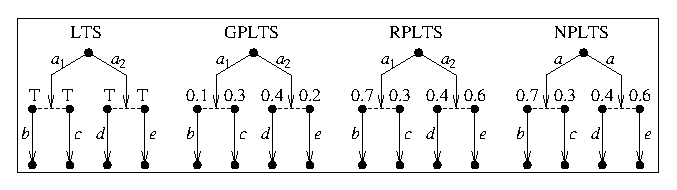
\includegraphics{figure/consumo_senza_ps}}
%%\caption{Consumo di energia senza power management}
%%\label{fig:consumo_senza_ps}
%\end{figure}
%
%Attivando il power management si pu\`o notare un sensibile risparmio energetico, a fronte di un diverso
%consumo energetico dovuto ad un diverso modo di operare: 
%
%\begin{figure}[htbp]
%%\centerline{\includegraphics{figure/consumo_con_ps}}
%%\caption{Consumo di energia con power management}
%%\label{fig:consumo_con_ps}
%\end{figure}
%
%In questa modalit\`a la stazione resta per la maggior parte del tempo nello stato di sleep, risvegliandosi
%periodicamente (nella figura ogni 100~ms) per controllare se nel frattempo c'\`e stato traffico per essa.
%Durante il periodo di sleep, sar\`a demandato all'Access Point il compito di bufferizzare i frame destinati
%verso la scheda momentaneamente in sleep; al risveglio i frame bufferizzati saranno annunciati da un {\em
%Beacon frame}, la ricezione da parte della stazione wireless dei frame bufferizzati inizier\`a subito dopo
%con la loro richiesta tramite il {\em PS-Poll frame} (Figura~\ref{fig:power_saving}).
%
%\begin{figure}[htbp]
%%\centerline{\includegraphics{figure/power_saving}}
%%\caption{Visione beacon e Ps-Poll}
%%\label{fig:power_saving}
%\end{figure}
%
%Quando viene attivato il power management l'Access Point e la stazione wireless devono sincronizzarsi per
%risvegliarsi ad intervalli prestabiliti, che nel caso della figura soprastante \`e 100~ms; all'inizio di
%ogni risveglio l'Access Point invier\`a il beacon contenente la {\em traffic indication map - TIM} che dice
%alla stazione se vi sono pacchetti bufferizzati destinati ad essa; in tal cosa la stazione risponder\`a con
%un PS-Pool contenente il suo Association ID. Grazie all'Association ID l'Access Point sar\`a in grado di
%selezionare i frame destinati alla stazione e provveder\`a ad inviarli.

\chapter{Scalabilit\'a, Pro e Contro}\label{cap:scalprocont}
\section{Scalabilit\'a}\label{sez:scalabilita}
Il problema della Scalabilit\'a, ossia della capacit\'a dell'applicazione di resistere all'aumentare del numero di utenti concorrenti che ne usufruiscono, dipende dal modello scelto, come anche dalla tipologia di applicazine sviluppata.
Non \'e quindi risolvibile banalmente e non esiste una scelta universalmente giusta.

Il problema della scalabilit\'a comunque \'e fondamentalmente diverso tra Blazor Server, e tutti gli altri modelli.
Questo principalmente per 3 motivi:
\begin{enumerate}
	\item Il primo \'e che Blazor Server delega completamente al Server che ospita l'applicazione il carico computazionale necessario per gestire ogni singolo evento della UI di ogni utente connesso, compreso il salvataggio in-memory  dello stato di ciascuna UI nel tempo durante l'utilizzo, visto che ad ogni Client connesso (o meglio allo specifico DOM) arrivano solamente le minime differenze necessarie rispettper generare la ui corretta rispetto al frame precedente, ogni volta che deve cambiare qualcosa.
	Ci\'o implica che la potenza del server debba tener conto di eventuali picchi di utenze, e debba avere a disposizione sufficiente RAM per poter mantenere in memoria lo stato dell'applicazione di ciascun utente concorrente connesso.
	
	\item Il secondo \'e che Blazor Server, necessita di una connessione sempre attiva con ogni utente collegato.
	
	\item Il terzo \'e che questo modello sfrutta SignalR, che per funzionare al meglio utilizza il protocollo di trasporto WebSocket, quindi la macchina server sul quale viene ospitata l'applicazione Blazor \'e consigliato che lo supporti.
\end{enumerate}

Gli altri modelli invece sfruttano l'hardware di ogni client connesso, come solitamente avviene per le SPA odierne.
Sono quindi in linea con il comportamento degli altri framework gi\'a citati e come Angular React o Vue.js, in particolare Blazor WebAssembly, che quindi prenderemo in considerazione confrontandolo con Blazor Server.

\section{Blazor Server}\label{sez:scalabilitaBServer}

\subsection{Pro}\label{sez:proBServer}

\subsection{Contro}\label{sez:controBServer}


\section{Blazor WebAssembly}\label{sez:scalabilitaBWA}

\subsection{Pro}\label{sez:proBWA}


\subsection{Contro}\label{sez:controBWA}
\chapter{Conclusioni}\label{cap:conclusioni}
\section{Conclusioni}\label{sez:conclusioni}
Questo studio, ha cercato di rispondere alla domanda: "Cos'\`e Blazor?".
A tal fine, \`e stato descritto prima di tutto quali siano le tecnologie utilizzate da questo framework che in parte cambiano a seconda del modello scelto.
\`E stata implementata una applicazione web sfruttando Blazor Server, e dove disponibili sono stati mostrati gli esempi disponibili per gli altri modelli.
Ci\`o \`e stato fatto per spiegare il diverso funzionamento, a seconda del modello scelto, con i pro e contro di ciascuno.
\`E emerso che non esiste una scelta universalmente giusta, poich\'e a seconda delle esigenze dell'applicazione da sviluppare, un modello pu\`o risultare pi\`u o meno adatto.

\section{Futuro del progetto}\label{sez:futuro}
\begin{figure}[H]
	\centerline{\includegraphics[scale=0.8]{figure/ModelsSupportedOrNot.png}}
	\caption{Modelli blazor e supporto}
	\label{fig:supportedBlazorModels}
\end{figure}

\begin{figure}[H]
	\centerline{\includegraphics[scale=0.6]{figure/BlazorModels.PNG}}
	\caption{Modelli attuali e futuri}
	\label{fig:blazorModels}
\end{figure}

Onbeforeunload

Server 

WebAssembly, promettente ma ancora interpretato, si dovrebbe tradurre .NET direttamente in WebAssembly e in modalità AOT per avere prestazioni ben migliori e giustificare il non utilizzo di JS.

In Roadmap
PWA solo su Chrome
Electron, bello ma molto pesante
Native --> la complessità non giustifica la scelta, al momento e un esercizio accademico.
\include{sorgenti/cap_5}

\appendix
%\include{sorgenti/app_a}
\begin{thebibliography}{999}

\bibitem{Hoff}
M.~Wanyoike,
Disponibile: https://blog.logrocket.com/history-of-frontend-frameworks.

\bibitem{jquery}
Disponibile: https://en.wikipedia.org/wiki/JQuery.

\bibitem{stackOverflow2019}
Disponibile:
https://insights.stackoverflow.com/survey/2019\#technology-\_-web-frameworks

\bibitem{vueJs}
Disponibile: https://it.wikipedia.org/wiki/Vue.js

\bibitem{razor}
R.~Anderson,
R.~Nowak,
Disponibile: https://docs.microsoft.com/en-us/aspnet/core/razor-pages/?view=aspnetcore-3.0\&tabs=visual-studio

\bibitem{blazorWikiGitHub}
Disponibile: https://github.com/aspnet/Blazor/wiki/FAQ\#q-where-does-the-name-blazor-come-from

\bibitem{SPA}
Disponibile: https://en.wikipedia.org/wiki/Single-page\_application

\bibitem{blazorServerRelease}
D.~Roth,
Disponibile: https://devblogs.microsoft.com/aspnet/asp-net-core-and-blazor-updates-in-net-core-3-0.

\bibitem{whatIsAComponent}
L.~Latham, D.~Roth
Disponibile: https://docs.microsoft.com/en-us/aspnet/core/blazor/components?view=aspnetcore-3.1

\bibitem{signalR}
Disponibile: https://dotnet.microsoft.com/apps/aspnet/signalr

\bibitem{signalR-ASP.NET}
https://docs.microsoft.com/en-us/aspnet/core/signalr/introduction?view=aspnetcore-3.1

\bibitem{blazorModelsScenarios}
D.~Roth,
Disponibile: https://devblogs.microsoft.com/aspnet/blazor-server-in-net-core-3-0-scenarios-and-performance.

\bibitem{webAssemblyOfficialWebsite}
Disponibile: https://webassembly.org/

\bibitem{webAssemblySupport}
Disponibile: https://webassembly.org/roadmap/

\bibitem{blazorPWA}
D.~Roth,
Disponibile:
https://youtu.be/qF6ixMjCzHA?t=485

\bibitem{electronWiki}
Disponibile:
https://en.wikipedia.org/wiki/Electron\_(software\_framework)

\bibitem{electronDotNet}
Disponibile: https://github.com/ElectronNET/Electron.NET/blob/master/README.md

\bibitem{sandersonNDCBlutter}
S.~Sanderson
Disponibile: https://www.aka.ms/blutter

\bibitem{blazorNative}
D.~Roth,
Disponibile: https://youtu.be/qF6ixMjCzHA?t=872

\bibitem{ryanNowakNDCSydney}
S.~Sanderson, R.~Nowak

Disponibile: https://www.youtube.com/watch?v=dCgqTDki-VM

\bibitem{bServerConcurrentUsersTest}
Disponibile: https://docs.microsoft.com/it-it/aspnet/core/host-and-deploy/blazor/server?view=aspnetcore-3.1\#deployment-server


%
%\bibitem{MathewsSicuranza}
%V.~J.~Mathews e G.~L.~Sicuranza,
%{\em Polynomial Signal Processing},
%New York: Wiley, 2000, pp.100-120.
%
%\bibitem{CariniMumoloSicuranza}
%A.~Carini, E.~Mumolo e G. L.~Sicuranza,
%``V-Vector Algebra and Volterra Filters'',
%in {\em Advances in Imaging \& Electron Physics}, Vol.~124,
%P.~W.~Hawkes, Ed., San Diego: Academic Press, 2003, pp.~1-61. 
%
%\bibitem{Carini}
%A.~Carini,
%``Efficient NLMS and RLS Algorithms for Perfect and Imperfect Periodic Sequences'',
%{\em IEEE Transactions on Signal Processing}, vol.~58, No.~4, pp.~2048-2059, Aprile 2010.
%
%\bibitem{CariniMathewsSicuranza}
%A.~Carini, V.~J.~Mathews e G.~L.~Sicuranza,
%``Efficient NLMS and RLS Algorithms for a Class of Nonlinear Filters Using Periodic Input Sequences'',
%{\em Proceedings of 36th International Conference on Acoustics, Speech, and Signal Processing, ICASSP 2011},
%Prague, Czech Republic, Maggio 22-27, 2011, pp.~4280-4283.
%
%\bibitem{CariniBrv}
%A.~Carini,
%``Filter for the Equalization and/or Linearization of Nonlinear Systems'',
%Brevetto Europeo EP~0939487A2, 25 Febbraio~1999.
%
%\bibitem{Standard}
%{\em IEEE Criteria for Class IE Electric Systems}, IEEE Standard 308, 1969.
%
%\bibitem{Jones}
%J.~Jones,
%{\em Networks} (2nd ed.) [Online] (10 Maggio 1991). [Ultimo accesso: 11 Maggio 2001].
%Disponibile: http://www.atm.com 

%\bibitem{Vidmar}
%R.~J.~Vidmar,
%{\em On the Use of Atmospheric Plasmas as Electromagnetic Reflectors} [Online]. (1994).
%[Ultimo accesso: 11 Maggio 2001]
%Disponibile FTP: atmnext.usc.edu Directory: pub/etext/1994 File: atmosplasma.txt

%\bibitem{Biglieri-84}
%E.~Biglieri, A.~Gersho, R.~D.~Gitlin and T.~L.~Lim, ``Adaptive Cancellation of Nonlinear Intersymbol
%Interference for Voiceband Data Transmission'', {\em IEEE Journal on Selected Areas in Communications},
%Vol.~SAC-2, No.~5, Sep.~1984, pp.~765-777.
%
%\bibitem{Biglieri-88}
%E.~Biglieri, S.~Barberis and M.~Catena, ``Analysis and Compensation of Nonlinearities in Digital
%Transmission Systems'', {\em IEEE Journal on Selected Areas in Communications}, Vol.~6, No.~1, Jan.~1988,
%pp.~42-51.
%
%\bibitem{Biglieri-89}
%E.~Biglieri, M.~Elia and L.~Lopresti, ``The Optimal Linear Receiving Filter for Digital Transmission Over
%Nonlinear Channels'', {\em IEEE Trans. on Information Theory}, Vol.~35, No.~3, May 1989, pp.~620-625.
%
%\bibitem{Biglieri-94}
%E.~Biglieri, E.~Chiaberto, G.P.~Maccone and E.~Viterbo, ``Compensation of Nonlinearities in High-Density
%Magnetic Recording Channels'', {\em IEEE Trans. on Magnetics}, Vol.~30, No.~6, Nov.~1994, pp.~5079-5086.
%
%\bibitem{bitmead-80}
%R.R.~Bitmead and B.D.O.~Anderson, ``Lyapunov Techniques for the Exponential Stability of Linear Difference
%Equations with Random Coefficients'', {\em IEEE Trans. on Automatic Control,} Vol.~AC-25, No.~4, Aug. 1980,
%pp.782-787.
%
%\bibitem{Bose-95}
%T.~Bose and D.A.~Trautman, ``Stability of the Quantized LMS Algorithm'', {\em Circuits Systems Signal
%Processing}, Vol.~14, No.~5, 1995, pp.~587-602.
%
%\bibitem{Bose-951}
%T.~Bose and M.~Q.~Chen, ``BIBO Stability of the Discrete Bilinear Systems'', {\em Digital Signal Processing:
%A Review Journal}, Vol.~5, No.~3, July 1995, pp.~160-166.
%
%\bibitem{Carini-95}
%A.~Carini and E.~Mumolo, ``A Novel Algebraic Formulation for the Development of Adaptive Volterra Filtering
%Algorithms'', {\em Proceedings of 1995 IEEE Workshop on Nonlinear Signal and Image Processing}, June 20-22
%1995, Neos Marmaras, Halkidiki, Greece, pp.~943-946.
%
%\bibitem{Carini-951}
%A.~Carini and E.~Mumolo, ``Adaptive Stabilization of Recursive Second Order Polynomial Filters by Means of a
%Stability Test'', {\em Proceedings of 1995 IEEE Workshop on Nonlinear Signal and Image Processing}, June
%20-22 1995, Neos Marmaras, Halkidiki, Greece, pp.~939-942.
%
%\bibitem{Carini-96}
%A.~Carini, ``A Novel Givens Rotation Based Fast SQR-RLS Algorithm'', {\em Proc. of EUSIPCO-96, VIII European
%Signal Processing Conference}, Trieste, Italy, September 10-13 1996, pp.~1235-1238.
%
%\bibitem{Carini-97}
%A.~Carini and E.~Mumolo, ``Fast Square-Root RLS Adaptive Filtering Algorithms'', {\em Signal Processing},
%Vol.~57, No.~3, Mar.~1997, pp.~233-250.
%
%\bibitem{Carini-971}
%A.~Carini, G.L.~Sicuranza and V.J.~Mathews, ``On the Inversion of Certain Nonlinear Systems'', {\em IEEE
%Signal Processing Letters}, Dec.~1997.

\end{thebibliography}


\ringraziamenti
Vorrei ringraziare il professor Lattanzi per avermi aiutato a scrivere questa tesi, i miei genitori per avermi permesso di procedere facendo di testa mia su un percorso a loro estraneo, e la mia ragazza Ivana per aver creduto in me e nelle mie capacit� anche quando non l'ho fatto io.

\end{document}
